% Provenance (never printed): see sources/outline_sources.md (Year 3:
% concordia and discordia; 40Ar/39Ar step heating; Sm-Nd model ages;
% cosmogenic nuclides; fission tracks and (U-Th)/He). Brief:
% sources/book5/BRIEFS.md, ch. 13. Curves from figdata/bachelor-3/
% concordia.py, arar_spectrum.py, model_ages.py, cosmogenic.py. Exercise and
% problem values in the Book 5 scratch calculator calc/ch13.py. The zircons,
% the biotite spectrum, the Nd sample and the helium ages of the Varden
% granite are invented, consistent with the Year 1 volume's granite of 310 Ma.
\chapter{उन्नत काल-निर्धारण}\label{ch:b3:advanced-geochronology}

ज़िरकॉन का एक क्रिस्टल, जो एक मिलीमीटर के दसवें भाग जितना लंबा है, अपने ग्रेनाइट के
क्रिस्टलीकृत होने के बाद से दो घड़ियाँ चला रहा है: यूरेनियम-238, जो सीसा-206 में क्षय होता है,
और यूरेनियम-235, जो सीसा-207 में क्षय होता है। जब दोनों घड़ियाँ एक ही आयु बताएँ, तो वह
आयु निस्संदेह होती है। जब वे असहमत हों, तो असहमति स्वयं काल-निर्धारित की जा सकती है: क्रिस्टल ने
किसी बाद की घटना में अपने सीसे का कुछ भाग खो दिया, और दोनों घड़ियाँ, साथ पढ़ी जाने पर, ग्रेनाइट की आयु और उस घटना की आयु देती हैं।
यह अध्याय एक साथ कई घड़ियाँ पढ़ता है: यूरेनियम और सीसे में,
आर्गन में, नियोडिमियम में, विखंडन-पथों और हीलियम में,
तथा ब्रह्मांडी किरणों द्वारा बने दुर्लभ परमाणुओं में,
और बताता है कि प्रत्येक आयु पर कितना भरोसा किया जा सकता है।

\begin{recall}
रेडियोधर्मी क्षय, आयु समीकरण, समकालरेखा और उसका आरंभिक अनुपात,
न्यूनतम वर्ग रेखा, शाखित क्षय, पोटैशियम--आर्गन आयु, अवरोध-तापमान
और शीतलन-आयु पुस्तक 3 (स्नातक वर्ष 1) में हैं, उसके रेडियोमीट्रिक काल-निर्धारण वाले अध्याय में;
ब्रह्मांडजनित नाभिकों का स्थायी-अपरदन सूत्र उसी पुस्तक के
अपरदन और परिवहन वाले अध्याय में है। कॉन्ड्राइटी एकसमान भंडार, एप्सिलॉन संकेतन
और क्षीणित प्रावार पुस्तक 4 (स्नातक वर्ष 2) में हैं, उसके समस्थानिक भू-रसायन वाले अध्याय में;
तापीय आयनन और बहु-संग्राहक द्रव्यमान स्पेक्ट्रममिति उसके क्षेत्र और प्रयोगशाला विधियों वाले अध्याय में
हैं। \omterm{def:b3:orogenic-wedges:thermochronology}{ऊष्मकालमिति} और
\omterm{def:b3:orogenic-wedges:age-elevation}{आयु--ऊँचाई संबंध} \cref{ch:b3:orogenic-wedges} में हैं।
\end{recall}

\section{यूरेनियम, सीसा और कॉन्कॉर्डिया}\label{sec:b3:advanced-geochronology:upb}

यूरेनियम के दो दीर्घजीवी समस्थानिक हैं। यूरेनियम-238 अल्पजीवी संतति नाभिकों की एक श्रृंखला से होकर
सीसा-206 में क्षय होता है, जिसका क्षय-स्थिरांक $\lambda_{238} =
\qty{1.55125e-10}{yr^{-1}}$ है; यूरेनियम-235 सीसा-207 में क्षय होता है, जिसका क्षय-स्थिरांक $\lambda_{235}
= \qty{9.8485e-10}{yr^{-1}}$ है, जो छह गुना तेज़ है। इनका वर्तमान अनुपात
$^{235}\mathrm{U}/^{238}\mathrm{U} = 0.0072567$ है, या $^{238}\mathrm{U}/^{235}\mathrm{U}
= 137.8$ है, और यह हर पार्थिव चट्टान में एक समान है। ज़िरकॉन, $\mathrm{ZrSiO_4}$, बढ़ते समय
बहुत यूरेनियम लेता है और लगभग कोई सीसा नहीं, अपक्षय का प्रतिरोध करता है
और कायांतरण से बच निकलता है: इसका लगभग सारा सीसा रेडियोजनित होता है।
% ledger: amherst:constants, tulane:upb-zircon

मान लीजिए $x = {}^{207}\mathrm{Pb}^*/{}^{235}\mathrm{U}$ और $y =
{}^{206}\mathrm{Pb}^*/{}^{238}\mathrm{U}$ ये रेडियोजनित सीसे के अपने जनक से वर्तमान अनुपात हैं। हर एक से एक आयु मिलती है, जैसे
$t_{206} = \ln(1 + y)/\lambda_{238}$,
और $t_{207} = \ln(1 + x)/\lambda_{235}$।

\begin{definition}[कॉन्कॉर्डिया, डिस्कॉर्डिया, अंतःखंड, टेरा--वासरबर्ग आरेख]
\label{def:b3:advanced-geochronology:concordia}
\emph{कॉन्कॉर्डिया}\index{कॉन्कॉर्डिया} $(x, y)$ तल का वह वक्र है, जिस पर
दोनों यूरेनियम--सीसा आयुएँ बराबर होती हैं। \emph{डिस्कॉर्डिया}\index{डिस्कॉर्डिया} वह सीधी रेखा है
जिसके अनुदिश एक ही क्रिस्टल-समष्टि के असंगत विश्लेषण
संरेखित होते हैं; कॉन्कॉर्डिया के साथ इसके प्रतिच्छेद बिंदु
\emph{ऊपरी अंतःखंड}\index{ऊपरी अंतःखंड} (अधिक पुराना) और
\emph{निचला अंतःखंड}\index{निचला अंतःखंड} (कम पुराना) कहलाते हैं।
\emph{टेरा--वासरबर्ग आरेख}\index{टेरा--वासरबर्ग आरेख} वह आरेख है जिसमें
$X = {}^{238}\mathrm{U}/{}^{206}\mathrm{Pb}^*$ को $Y =
{}^{207}\mathrm{Pb}^*/{}^{206}\mathrm{Pb}^*$ के विरुद्ध आलेखित किया जाता है।
\end{definition}

\begin{theorem}[कॉन्कॉर्डिया]\label{thm:b3:advanced-geochronology:concordia}
एक क्रिस्टल, जो बनने के बाद से यूरेनियम और सीसे के लिए एक बंद तंत्र रहा है,
और $t$ समय पहले बना, इस बिंदु पर आलेखित होता है:
\[
C(t) = \bigl(e^{\lambda_{235}t} - 1,\; e^{\lambda_{238}t} - 1\bigr).
\]
जैसे-जैसे $t$ बढ़ता है, वक्र $x$ के सापेक्ष अधिकाधिक धीमी गति से ऊपर उठता है: इसकी प्रवणता,
$\mathrm dy/\mathrm dx = (\lambda_{238}/\lambda_{235})\,e^{(\lambda_{238} -
\lambda_{235})t}$ घटती है, मूल बिंदु पर $\lambda_{238}/\lambda_{235} = 0.1575$ से
अतः \omterm{def:b3:advanced-geochronology:concordia}{कॉन्कॉर्डिया} $x$ अक्ष की ओर अवतल है।
\end{theorem}

\begin{proof}
प्रत्येक जनक के लिए, प्रति जनक परमाणु शेष रेडियोजनित संतति परमाणुओं की संख्या
$e^{\lambda t} - 1$ है, जो पुस्तक 3 (स्नातक वर्ष 1) का आयु समीकरण है।
दोनों निर्देशांकों का $t$ के सापेक्ष अवकलन करके और भाग देने पर प्रवणता मिलती है; चूँकि
$\lambda_{235} > \lambda_{238}$ है, इसलिए यह $t$ के साथ घटती है।
\end{proof}

सीसा एक बड़ा आयन है जो ज़िरकॉन की जालक में ठीक से नहीं बैठता। क्रिस्टल के उन भागों में,
जो अपनी ही रेडियोधर्मिता से क्षतिग्रस्त हैं, वहाँ से सीसा किसी बाद की
तापन या तरल परिसंचरण की घटना में निकल सकता है।
% ledger: tulane:upb-zircon

\begin{theorem}[सीसे की रुक-रुककर होने वाली हानि एक जीवा देती है]\label{thm:b3:advanced-geochronology:discordia}
एक क्रिस्टल, जो $t_1$ समय पहले बना और $t_2$ समय पहले
अपने रेडियोजनित सीसे का अंश $f$ खो बैठा और अन्यथा बंद रहा, आज इस बिंदु पर आलेखित होता है:
\[
(1 - f)\,C(t_1) + f\,C(t_2),
\]
\omterm{def:b3:advanced-geochronology:concordia}{कॉन्कॉर्डिया} के बिंदुओं $t_1$ और $t_2$ को मिलाने वाली जीवा पर स्थित होता है। भिन्न-भिन्न अंश खोने वाले क्रिस्टल
उसी जीवा पर पड़ते हैं, जो एक \omterm{def:b3:advanced-geochronology:concordia}{डिस्कॉर्डिया} है जिसका \omterm{def:b3:advanced-geochronology:concordia}{ऊपरी
अंतःखंड} $t_1$ है और \omterm{def:b3:advanced-geochronology:concordia}{निचला अंतःखंड} $t_2$।
\end{theorem}

\begin{proof}
मान लीजिए एक क्षय-तंत्र है, जिसका स्थिरांक $\lambda$ है, और आज विद्यमान जनक के
प्रति परमाणु गिनी जाती है। $t_2$ समय पहले $e^{\lambda t_2}$ जनक परमाणु थे, और
रेडियोजनित संतति $e^{\lambda t_2}(e^{\lambda(t_1 - t_2)} - 1) =
e^{\lambda t_1} - e^{\lambda t_2}$ थी। घटना के बाद $(1 - f)(e^{\lambda t_1} -
e^{\lambda t_2})$ शेष रहा; तब से जनक ने $e^{\lambda t_2} - 1$ और संतति नाभिक बनाए।
योग $(1 - f)(e^{\lambda t_1} - 1) + f(e^{\lambda t_2} - 1)$ है। सीसे के दोनों
समस्थानिक रासायनिक रूप से एक जैसा व्यवहार करते हैं, अतः $f$ दोनों के लिए एक ही है, और दोनों
निर्देशांक मिलकर ऊपर कहा गया बिंदु देते हैं।
\end{proof}

\begin{omfigure}
\begin{tikzpicture}
\begin{groupplot}[group style={group size=2 by 1, horizontal sep=1.7cm},
  omrecord, width=0.47\linewidth, height=0.42\linewidth, title style={font=\small},
  tick label style={font=\scriptsize}, label style={font=\small}]
\nextgroupplot[title={(क) कॉन्कॉर्डिया आरेख},
  xlabel={$^{207}\mathrm{Pb}^*/^{235}\mathrm{U}$}, ylabel={$^{206}\mathrm{Pb}^*/^{238}\mathrm{U}$},
  xmin=0.04, xmax=0.44, ymin=0.006, ymax=0.06,
  xtick={0.1,0.2,0.3,0.4}, xticklabels={0.1,0.2,0.3,0.4},
  ytick={0.01,0.02,0.03,0.04,0.05}, yticklabels={0.01,0.02,0.03,0.04,0.05},
  scaled ticks=false]
% computed in figdata/bachelor-3/concordia.py
\addplot[black, thick] table[x=xw, y=yw] {figdata/out/bachelor-3-concordia-curve.dat};
\addplot[black, only marks, mark=*, mark size=1.4pt, nodes near coords={\scriptsize\pgfmathprintnumber[fixed, precision=0]{\pgfplotspointmeta}},
  point meta=explicit, nodes near coords align={anchor=south east},
  restrict expr to domain={\thisrow{t}}{100:350}]
  table[x=xw, y=yw, meta=t] {figdata/out/bachelor-3-concordia-ticks.dat};
\addplot[omDef, thick, densely dashed] table[x=x, y=y] {figdata/out/bachelor-3-concordia-line.dat};
\addplot[red!70!black, only marks, mark=diamond*, mark size=2pt] table[x=x, y=y] {figdata/out/bachelor-3-concordia-zircons.dat};
\nextgroupplot[title={(ख) टेरा--वासरबर्ग आरेख},
  xlabel={$^{238}\mathrm{U}/^{206}\mathrm{Pb}^*$}, ylabel={$^{207}\mathrm{Pb}^*/^{206}\mathrm{Pb}^*$},
  xmin=15, xmax=75, ymin=0.0465, ymax=0.0535,
  ytick={0.047,0.049,0.051,0.053}, yticklabels={0.047,0.049,0.051,0.053},
  scaled ticks=false]
\addplot[black, thick] table[x=xtw, y=ytw] {figdata/out/bachelor-3-concordia-curve.dat};
\addplot[black, only marks, mark=*, mark size=1.4pt, nodes near coords={\scriptsize\pgfmathprintnumber[fixed, precision=0]{\pgfplotspointmeta}},
  point meta=explicit, nodes near coords align={anchor=north east},
  restrict expr to domain={\thisrow{t}}{100:250}]
  table[x=xtw, y=ytw, meta=t] {figdata/out/bachelor-3-concordia-ticks.dat};
\addplot[omDef, thick, densely dashed] table[x=xtw, y=ytw] {figdata/out/bachelor-3-concordia-twline.dat};
\addplot[red!70!black, only marks, mark=diamond*, mark size=2pt] table[x=xtw, y=ytw] {figdata/out/bachelor-3-concordia-zircons.dat};
\end{groupplot}
\end{tikzpicture}

\par\smallskip{\small (क) \omterm{def:b3:advanced-geochronology:concordia}{कॉन्कॉर्डिया}, जिस पर उसके आयु-मान लाखों वर्षों में दिए गए हैं,
और एक ही ग्रेनाइट के पाँच काल्पनिक असंकेंद्रीय ज़िरकॉन (लाल; उनके त्रुटि
दीर्घवृत्त चिह्नों से छोटे हैं), जो एक \omterm{def:b3:advanced-geochronology:concordia}{डिस्कॉर्डिया} (डैश वाली) पर संरेखित हैं,
वह रेखा \omterm{def:b3:advanced-geochronology:concordia}{कॉन्कॉर्डिया} को लगभग 311 और \qty{100}{\Ma} के पास काटती है। (ख) वही ज़िरकॉन और रेखा
\omterm{def:b3:advanced-geochronology:concordia}{टेरा--वासरबर्ग आरेख} में, जहाँ \omterm{def:b3:advanced-geochronology:concordia}{डिस्कॉर्डिया} अभी भी सीधी
रेखा रहती है।}\label{fig:b3:advanced-geochronology:concordia}
\end{omfigure}
% ledger: amherst:constants

अंतःखंड वहाँ पाए जाते हैं जहाँ $a + b\,x(t) = y(t)$ होता है, यह $t$ में एक समीकरण है
जिसे न्यूटन की विधि से हल किया जाता है: यहाँ $g(t) = e^{\lambda_{238}t} - 1 - a -
b(e^{\lambda_{235}t} - 1)$ और $g'(t) = \lambda_{238}e^{\lambda_{238}t} -
b\lambda_{235}e^{\lambda_{235}t}$ लेकर प्रत्येक अंतःखंड के पास के एक अनुमान से शुरू करके $t \leftarrow t - g/g'$
की पुनरावृत्ति की जाती है। परिणाम के तीन गुण व्यवहार में महत्त्वपूर्ण हैं।
पहला, \omterm{def:b3:advanced-geochronology:concordia}{ऊपरी अंतःखंड} तभी सटीक होता है जब \omterm{def:b3:advanced-geochronology:concordia}{डिस्कॉर्डिया} \omterm{def:b3:advanced-geochronology:concordia}{कॉन्कॉर्डिया} को
बड़े कोण पर काटती है। एक युवा \omterm{def:b3:advanced-geochronology:concordia}{डिस्कॉर्डिया}, जैसा ऊपर के चित्र में है, लगभग
\omterm{def:b3:advanced-geochronology:concordia}{कॉन्कॉर्डिया} के साथ-साथ चलती है, और उसकी ढाल में थोड़ा-सा परिवर्तन अंतःखंड को
बहुत दूर खिसका देता है। दूसरा, यदि सीसा-हानि हाल की है, $t_2 = 0$, तो \omterm{def:b3:advanced-geochronology:concordia}{डिस्कॉर्डिया}
मूल बिंदु से होकर गुज़रती है, और हर क्रिस्टल का वही
$^{207}\mathrm{Pb}^*/^{206}\mathrm{Pb}^*$ अनुपात होता है,
\[
\frac{^{207}\mathrm{Pb}^*}{^{206}\mathrm{Pb}^*} = \frac{1}{137.8}\,
\frac{e^{\lambda_{235}t_1} - 1}{e^{\lambda_{238}t_1} - 1},
\]
जो यूरेनियम के बिना $t_1$ देता है: यह सीसा--सीसा आयु है। तीसरा, \omterm{def:b3:advanced-geochronology:concordia}{कॉन्कॉर्डिया} आरेख में एक रेखा
$x = (y - a)/b$, टेरा--वासरबर्ग निर्देशांकों में
$Y = (1 - aX)/(137.8\,b)$ बन जाती है, जो फिर एक रेखा है। \omterm{def:b3:advanced-geochronology:concordia}{टेरा--वासरबर्ग
आरेख} सीधे मापे गए अनुपात लेता है, और उसमें यूरेनियम-235 की गणना यूरेनियम-238 से करने की
आवश्यकता नहीं होती, और सामान्य सीसे का एक मिश्रण, जो अविकिरणजनित है और
सीसा-207 से समृद्ध है, एक ऐसी रेखा पर अंकित होता है जो $Y$ अक्ष को सामान्य
सीसे के अनुपात पर काटती है।

यूरेनियम--सीसा आयु दो प्रकार से मापी जाती है। एकल क्रिस्टल या टुकड़े,
जिन्हें क्षतिग्रस्त क्षेत्र हटाने के लिए आंशिक विलयन के बाद घोला जाता है,
और जिनका सीसा तथा यूरेनियम अलग किया जाता है, उन्हें तापीय आयनन
द्रव्यमान स्पेक्ट्रममिति से मापा जाता है, जो भूविज्ञान की सबसे सटीक आयु देती है। कुछ दसियों
माइक्रोमीटर चौड़े धब्बे स्थान पर ही आयन प्रोब या लेज़र अपक्षरण से मापे जाते हैं,
कम सटीकता से, परंतु उस क्रिस्टल में क्षेत्र-दर-क्षेत्र, जो
कई घटनाओं में बढ़ा हो।

\begin{inthelab}[काल-निर्धारण प्रयोगशाला]
\begin{minipage}[t]{0.55\linewidth}\vspace{0pt}
एक ज़िरकॉन की तिथि एक कुचली हुई चट्टान से शुरू होती है और एक स्वच्छ प्रयोगशाला में समाप्त होती है। भूकालवैज्ञानिक
ज़िरकॉन को घनत्व और चुंबकत्व से अलग करते हैं, द्विनेत्री सूक्ष्मदर्शी के नीचे
सबसे स्पष्ट क्रिस्टल चुनते हैं और उनके क्षेत्रीकरण का चित्र लेते हैं। क्षतिग्रस्त क्षेत्र हटाने के लिए क्रिस्टलों को
आंशिक रूप से घोला जाता है, फिर ज्ञात समस्थानिकों के एक स्पाइक के साथ
पूरी तरह घोला जाता है, और यूरेनियम तथा सीसे को
रेज़िन के छोटे स्तंभों पर अलग किया जाता है, उस वायु में जो धूल के सीसे को
दूर रखने के लिए छानी गई हो। एक द्रव्यमान स्पेक्ट्रममापी समस्थानिक अनुपात मापता है। आर्गन के नमूने एक
अलग मार्ग पर चलते हैं: एक रिएक्टर, फिर एक गैस लाइन, जहाँ लेज़र हर चरण को गरम करता है और
स्पेक्ट्रममापी से पहले आर्गन साफ़ किया जाता है।
\end{minipage}\hfill
\begin{minipage}[t]{0.42\linewidth}\vspace{0pt}
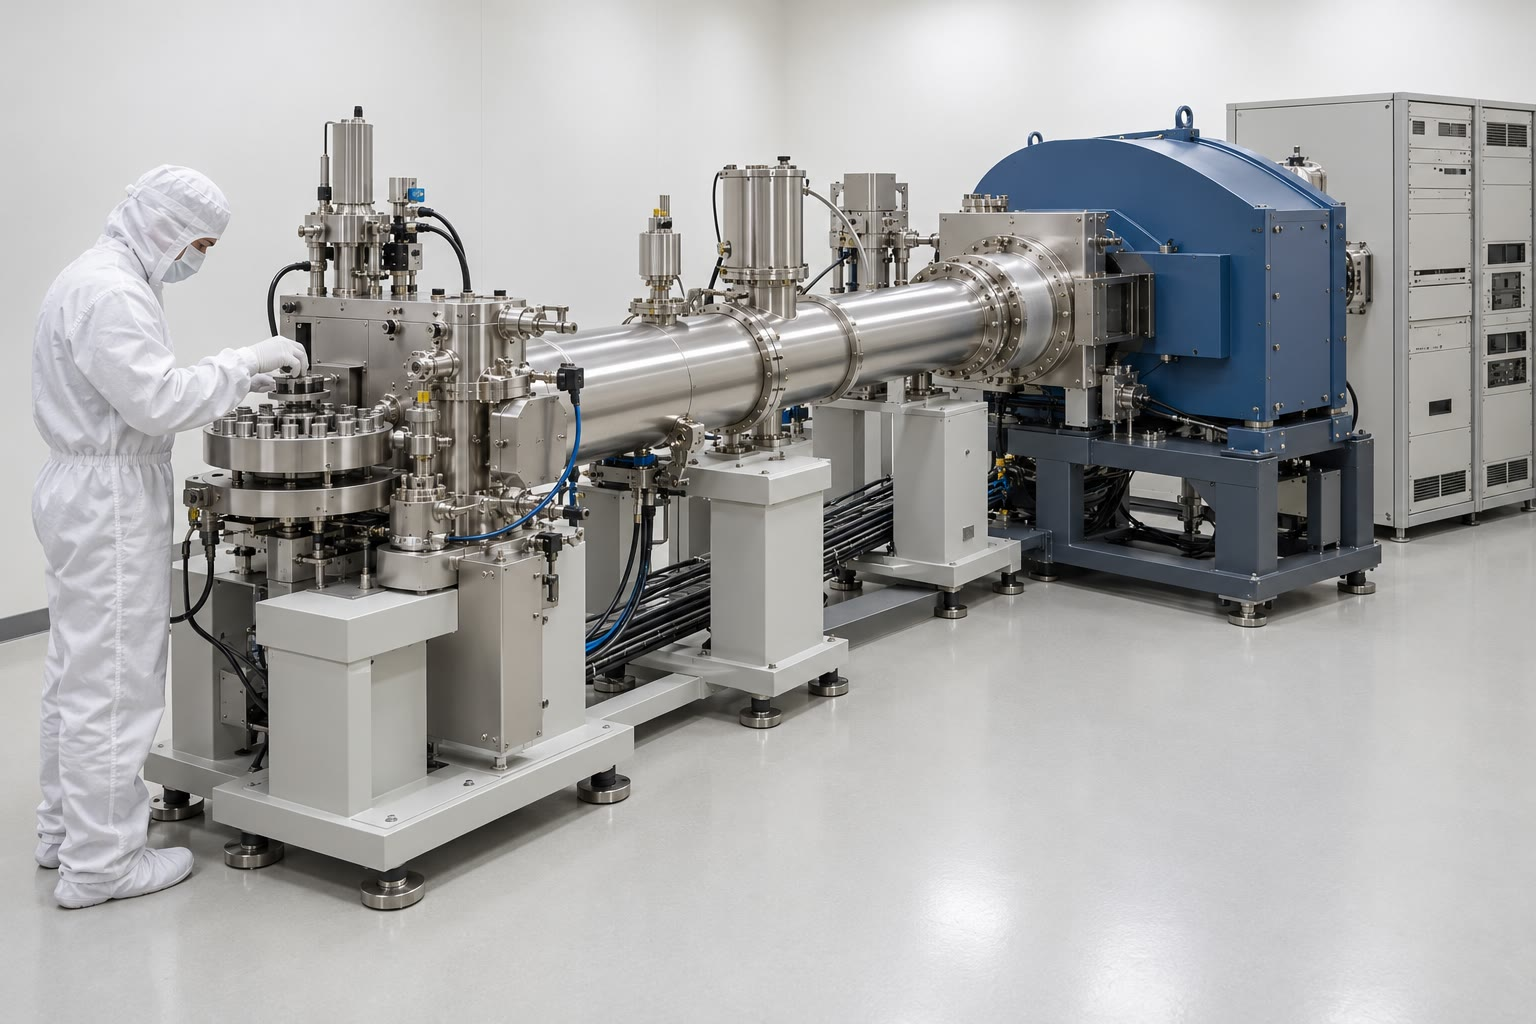
\includegraphics[width=\linewidth]{images/book5/ai/b3-mass-spec-lab.jpg}

{\scriptsize एक स्वच्छ प्रयोगशाला में द्रव्यमान स्पेक्ट्रममापी: बाईं ओर नमूना चक्री, उड़ान
नली और विद्युत-चुंबक (AI से बनाया गया
चित्रण)।}
\end{minipage}
\end{inthelab}

\section{आर्गन--आर्गन काल-निर्धारण}\label{sec:b3:advanced-geochronology:arar}

पुस्तक 3 की पोटैशियम--आर्गन विधि पोटैशियम और
आर्गन को एक खनिज के दो अलग-अलग अंशों में मापती है। आर्गन--आर्गन
विधि केवल आर्गन को, एक ही अंश में, समस्थानिक अनुपातों के रूप में मापती है। नमूने को
परमाणु रिएक्टर के कोर में तेज़ न्यूट्रॉनों से विकिरणित किया जाता है, जहाँ
अभिक्रिया $^{39}\mathrm{K}(n,p)^{39}\mathrm{Ar}$ उसके पोटैशियम-39 के एक निश्चित अंश को
आर्गन-39 में बदल देती है, जो पोटैशियम की प्रॉक्सी है। एक ज्ञात आयु का खनिज,
मॉनिटर, उसके बगल में विकिरणित किया जाता है।
% ledger: nmgrl:arar, amherst:arar

\begin{definition}[आर्गन--आर्गन काल-निर्धारण, J गुणक, आयु स्पेक्ट्रम, पठार आयु]
\label{def:b3:advanced-geochronology:arar}
\emph{$^{40}\mathrm{Ar}/^{39}\mathrm{Ar}$ काल-निर्धारण}\index{आर्गन--आर्गन काल-निर्धारण@$^{40}\mathrm{Ar}/^{39}\mathrm{Ar}$ काल-निर्धारण}
पोटैशियम-युक्त खनिज का काल-निर्धारण, अनुपात $R =
{}^{40}\mathrm{Ar}^*/{}^{39}\mathrm{Ar}_{\mathrm K}$ से होता है, यह अनुपात उसके रेडियोजनित
आर्गन-40 और न्यूट्रॉन विकिरण से उसके पोटैशियम से बने आर्गन-39 का है।
\emph{J गुणक}\index{J गुणक} किसी विकिरण का $J = (e^{\lambda
t_m} - 1)/R_m$ है, जो ज्ञात आयु $t_m$ वाले एक मॉनिटर और मापे गए अनुपात $R_m$ से ज्ञात होता है,
जहाँ $\lambda$ पोटैशियम-40 का कुल क्षय-स्थिरांक है। जब नमूने को
बढ़ते तापमान के चरणों में गैसरहित किया जाता है, तो उसका \emph{आयु
स्पेक्ट्रम}\index{आयु स्पेक्ट्रम} हर चरण की आयु को मुक्त हुए आर्गन-39 के संचयी
अंश के विरुद्ध दर्शाता है। \emph{पठार
आयु}\index{पठार आयु} लगातार उन चरणों की भारित माध्य आयु है जो
अपनी अनिश्चितताओं के भीतर मेल खाते हैं और आर्गन-39 का बड़ा भाग मुक्त करते हैं।
\end{definition}

\begin{theorem}[आर्गन--आर्गन आयु]\label{thm:b3:advanced-geochronology:arar}
एक नमूना, जिसे एक मॉनिटर के साथ विकिरणित किया गया है, की आयु इस प्रकार होती है:
\[
t = \frac1\lambda\ln(1 + JR).
\]
\end{theorem}

\begin{proof}
रेडियोजनित आर्गन $^{40}\mathrm{Ar}^* = (\lambda_e/\lambda)\,
{}^{40}\mathrm{K}\,(e^{\lambda t} - 1)$ है, पुस्तक 3 के शाखित क्षय के
अनुसार। बना हुआ आर्गन-39 $^{39}\mathrm{Ar}_{\mathrm K} =
{}^{39}\mathrm{K}\,\Phi$ है, जहाँ $\Phi$ न्यूट्रॉन खुराक और अभिक्रिया के
अनुप्रस्थ काट को समाहित करता है। अतः $R = (e^{\lambda t} - 1)/J$ है, जहाँ $J =
\lambda\,\Phi\,{}^{39}\mathrm{K}/(\lambda_e\,{}^{40}\mathrm{K})$। अनुपात
$^{40}\mathrm{K}/^{39}\mathrm{K}$ सभी पोटैशियम में समान है, और $\Phi$
साथ-साथ विकिरणित दो नमूनों के लिए समान है, इसलिए $J$ नमूने के लिए
और मॉनिटर के लिए भी; मॉनिटर की आयु और अनुपात से वह ज्ञात होता है, और $R$ को
उलटने पर $t$ प्राप्त होता है।
\end{proof}

नियतांक पोटैशियम--आर्गन विधि के हैं, $\lambda =
\qty{5.543e-10}{yr^{-1}}$। एक सामान्य मॉनिटर एक ज्वालामुखीय टफ़ा का सैनिडीन है, जिसकी आयु
\qty{28.201}{\Ma} है; मॉनिटर अनुपात $R_m = 1.3129$ से $J =
0.01200$ प्राप्त होता है। वायुमंडलीय आर्गन, जिसका $^{40}\mathrm{Ar}/^{36}\mathrm{Ar} = 295.5$ है,
हर चरण में मापे गए आर्गन-36 से घटाया जाता है, और कैल्सियम तथा स्वयं पोटैशियम से
न्यूट्रॉनों द्वारा बना आर्गन उसी पैकेट में विकिरणित लवणों से
सुधारा जाता है।
% ledger: schaen20:monitors, amherst:constants, nmgrl:arar

स्टेप हीटिंग इस विधि की सबसे बड़ी शक्ति है। नमूने को एक भट्टी में
या लेज़र से बढ़ते तापमान के चरणों में गर्म किया जाता है, और हर चरण से एक आयु प्राप्त होती है।
यदि खनिज अपने ठंडे होने के बाद से बंद रहा है, तो सभी चरण मेल खाते हैं: स्पेक्ट्रम
समतल होता है। यदि उसने अपने कणों की बाहरी परतों से आर्गन खोया है, तो पहले चरण,
जो बाहरी परतों से आते हैं, कम आयु के होते हैं, और आयुएँ सीढ़ी की तरह बढ़ती हुई एक
पठार की ओर जाती हैं, जिसे अंदरूनी भाग देते हैं। पठार के लिए अनुशंसित मानदंड यह हैं कि
कम से कम पाँच लगातार चरण हों, जिनमें आर्गन-39 का \qty{50}{\percent} से अधिक हिस्सा हो,
और उनके बीच कोई प्रवृत्ति न हो; सीढ़ी के निम्न-तापमान चरणों को सामान्यतः
विकिरणजनित आर्गन की हानि माना जाता है। अतिरिक्त आर्गन, जो खनिज के बनते समय किसी तरल से फँसा हो,
इसका उल्टा असर डालता है: वह कुछ चरणों को अधिक पुराना बना देता है, अक्सर पहले
और अंतिम चरणों को, जिससे स्पेक्ट्रम काठी के आकार का हो जाता है। सभी चरणों का योग, यानी कुल-गैस आयु,
वही होती जो पोटैशियम--आर्गन आयु देती: वह एक ऐसा माध्य है
जो इतिहास को छिपा देता है।
% ledger: schaen20:plateau, nmgrl:arar

\begin{omfigure}
\begin{tikzpicture}
\begin{groupplot}[group style={group size=2 by 1, horizontal sep=1.5cm},
  omrecord, height=0.38\linewidth, title style={font=\small},
  xlabel={संचयी $^{39}\mathrm{Ar}$ मुक्त (\unit{\percent})},
  tick label style={font=\scriptsize}, label style={font=\small}]
\nextgroupplot[title={(क) पूरा स्पेक्ट्रम}, width=0.52\linewidth,
  ylabel={स्पष्ट आयु (\unit{\Ma})}, xmin=0, xmax=100, ymin=130, ymax=320,
  xtick={0,20,40,60,80,100}, ytick={150,200,250,300}]
% computed in figdata/bachelor-3/arar_spectrum.py
\addplot[omDef, thick] table[x=cum, y=age] {figdata/out/bachelor-3-arar_spectrum-boxes.dat};
\node[font=\scriptsize, anchor=west] at (axis cs:12,180) {आर्गन हानि};
\node[font=\scriptsize, anchor=north, red!70!black] at (axis cs:59,290) {पठार};
\nextgroupplot[title={(ख) पठार, विस्तृत}, width=0.44\linewidth,
  xmin=15, xmax=100, ymin=290, ymax=300, xtick={20,40,60,80,100},
  ytick={290,292,294,296,298,300}]
\addplot[name path=hi, draw=none, forget plot] table[x=cum, y=hi] {figdata/out/bachelor-3-arar_spectrum-boxes.dat};
\addplot[name path=lo, draw=none, forget plot] table[x=cum, y=lo] {figdata/out/bachelor-3-arar_spectrum-boxes.dat};
\addplot[omDef!25, forget plot] fill between[of=hi and lo];
\addplot[omDef, thick] table[x=cum, y=age] {figdata/out/bachelor-3-arar_spectrum-boxes.dat};
\draw[red!70!black, thick] (axis cs:18,296.1) -- (axis cs:100,296.1);
\node[font=\scriptsize, anchor=south, red!70!black] at (axis cs:59,290.3) {पठार \qty[separate-uncertainty=true]{296.1 \pm 0.8}{\Ma}};
\end{groupplot}
\end{tikzpicture}

\par\smallskip{\small पहले चित्र के ग्रेनाइट के एक बायोटाइट का काल्पनिक \omterm{def:b3:advanced-geochronology:arar}{आयु स्पेक्ट्रम}:
हर चरण को उसकी आयु पर खींचा गया है, और उसकी चौड़ाई उस आर्गन-39 के हिस्से के अनुसार है
जो उसने मुक्त किया। (क) तीन निम्न-तापमान चरण सीढ़ी की तरह बढ़कर एक
पठार तक पहुँचते हैं। (ख) सात पठार चरण, जिनमें आर्गन-39 का \qty{82}{\percent} है,
उनकी दो-मानक-विचलन सीमाएँ (छायांकित) और \omterm{def:b3:advanced-geochronology:arar}{पठार
आयु} (लाल)।}\label{fig:b3:advanced-geochronology:spectrum}
\end{omfigure}

\section{नियोडिमियम मॉडल आयु}\label{sec:b3:advanced-geochronology:model-age}

जब प्रावार से एक गलित निकलकर महाद्वीपीय भूपर्पटी बनाता है, तो सैमेरियम,
जो अधिक संगत है, नियोडिमियम की तुलना में अधिक मात्रा में पीछे रह जाता है: नई भूपर्पटी का
$^{147}\mathrm{Sm}/^{144}\mathrm{Nd}$ अपने स्रोत से कम होता है, लगभग 0.13, अधिकांश
भूपर्पटी चट्टानों में, जबकि कॉन्ड्राइटी भंडार के लिए 0.1966 है। इसका
$^{143}\mathrm{Nd}/^{144}\mathrm{Nd}$ तब धीरे बढ़ता है। एक बार बनने के बाद, एक
भूपर्पटी की चट्टान अपना सैमेरियम--नियोडिमियम अनुपात बनाए रखती है, अपरदन, अवसादन
और यहाँ तक कि पुनः गलन के बावजूद, इसलिए उसका नियोडिमियम याद रखता है
कि वह प्रावार से कब निकला था।
% ledger: white08:model-age, white:chur

\begin{definition}[मॉडल आयु]\label{def:b3:advanced-geochronology:model-age}
किसी समस्थानिक तंत्र में एक चट्टान की \emph{मॉडल आयु}\index{मॉडल आयु} वह समय है
जिस पर उसका अनुपात, उसके वर्तमान जनक--पुत्री अनुपात से पीछे की ओर प्रक्षेपित करने पर,
एक मॉडल भंडार के अनुपात के बराबर होता है। नियोडिमियम के लिए $T_{\mathrm{CHUR}}$
कॉन्ड्राइटी एकसमान भंडार का उपयोग करता है, और $T_{\mathrm{DM}}$
क्षीणित प्रावार का।
\end{definition}

\begin{theorem}[मॉडल आयु]\label{thm:b3:advanced-geochronology:model-age}
एक नमूना, जिसके वर्तमान अनुपात $I_s = {}^{143}\mathrm{Nd}/^{144}\mathrm{Nd}$ और
$R_s = {}^{147}\mathrm{Sm}/^{144}\mathrm{Nd}$ हैं, और एक भंडार की तुलना में, जिसके
वर्तमान अनुपात $I_m$ और $R_m$ हैं, उसकी \omterm{def:b3:advanced-geochronology:model-age}{मॉडल आयु} इस प्रकार होती है:
\[
T = \frac1\lambda\ln\left(1 + \frac{I_s - I_m}{R_s - R_m}\right),
\qquad \lambda = \lambda_{147}.
\]
\end{theorem}

\begin{proof}
एक बंद तंत्र का, समय $T$ पहले, अनुपात $I - R(e^{\lambda T} - 1)$ था:
समकालरेखा समीकरण को पीछे की ओर पढ़ने पर। नमूने और भंडार के लिए इसे बराबर रखने पर
$I_s - I_m = (R_s - R_m)(e^{\lambda T} - 1)$ प्राप्त होता है।
\end{proof}

$\lambda_{147} = \qty{6.524e-12}{yr^{-1}}$ लेने पर भंडार ये हैं: कॉन्ड्राइटी भंडार,
जिसका आज का मान 0.512638 और 0.1966 है, और क्षीणित प्रावार, जिसका आज का मान
0.51315 है, लगभग $\varepsilon_{\mathrm{Nd}} = +10$; कॉन्ड्राइटी मानों से
\qty{4.55}{\Ga} पहले से एक बंद विकास यह अनुपात देता है
$^{147}\mathrm{Sm}/^{144}\mathrm{Nd} = 0.2137$। एक काल्पनिक ग्रेनाइट, जिसके
$I_s = 0.511900$ और $R_s = 0.1100$ हैं, उसका आज का $\varepsilon_{\mathrm{Nd}} = -14.4$ है,
आज $T_{\mathrm{CHUR}} = \qty{1.30}{\Ga}$ और $T_{\mathrm{DM}} =
\qty{1.84}{\Ga}$। नीचे का चित्र दोनों को पढ़ता है। क्षीणित-प्रावार आयु बेहतर आकलन है,
क्योंकि भूपर्पटी ऐसे प्रावार से निकाली गई है जो पहले से क्षीणित था;
यह वह माध्य आयु है जिस पर नमूने का नियोडिमियम प्रावार से निकला;
यह उसकी भूपर्पटी में निवास आयु है। इसकी दो सीमाएँ हैं: भूपर्पटी को उसके बाद से
अपना सैमेरियम--नियोडिमियम अनुपात नहीं बदलना चाहिए, और वह चट्टान जो
पुरानी भूपर्पटी को नए प्रावार गलित के साथ मिलाकर बनी हो, उसकी मध्यवर्ती \omterm{def:b3:advanced-geochronology:model-age}{मॉडल आयु} निरर्थक होती है।
% ledger: villa20:sm147, white:chur, white08:model-age

\begin{omfigure}
\begin{tikzpicture}
\begin{axis}[omrecord, width=0.72\linewidth, height=0.38\linewidth,
  xlabel={वर्तमान से पहले का समय (\unit{\Ga})}, ylabel={$\varepsilon_{\mathrm{Nd}}$},
  xmin=0, xmax=2.5, ymin=-17, ymax=13, x dir=reverse,
  xtick={0,0.5,1,1.5,2,2.5}, xticklabels={0,0.5,1,1.5,2,2.5},
  tick label style={font=\scriptsize}, label style={font=\small},
  legend style={font=\scriptsize, at={(0.5,1.03)}, anchor=south, legend columns=3, legend cell align=left}]
% computed in figdata/bachelor-3/model_ages.py
\addplot[omDef, thick] table[x=t, y=eps_dm] {figdata/out/bachelor-3-model_ages-evolution.dat};
\addlegendentry{क्षीणित प्रावार}
\addplot[black, thick, densely dashed] coordinates {(0,0) (2.5,0)};
\addlegendentry{CHUR}
\addplot[red!70!black, thick] table[x=t, y=eps_sample] {figdata/out/bachelor-3-model_ages-evolution.dat};
\addlegendentry{ग्रेनाइट}
\draw[densely dotted] (axis cs:1.30,0) -- (axis cs:1.30,-17) node[above right, font=\scriptsize, rotate=90] {$T_{\mathrm{CHUR}}$};
\draw[densely dotted] (axis cs:1.84,5.4) -- (axis cs:1.84,-17) node[above right, font=\scriptsize, rotate=90] {$T_{\mathrm{DM}}$};
\end{axis}
\end{tikzpicture}

\par\smallskip{\small $\varepsilon_{\mathrm{Nd}}$ एक काल्पनिक ग्रेनाइट का,
जिसे उसके अपने समैरियम--नियोडिमियम अनुपात से समय में पीछे प्रक्षेपित किया गया (लाल)। यह
$T_{\mathrm{CHUR}} = \qty{1.30}{\Ga}$ पर कॉन्ड्राइटी भंडार से और
$T_{\mathrm{DM}} = \qty{1.84}{\Ga}$ पर क्षीणित प्रावार (नीला) से मिलता है।}\label{fig:b3:advanced-geochronology:model-age}
\end{omfigure}

\section{विखंडन-पथ और हीलियम}\label{sec:b3:advanced-geochronology:low-t}

यूरेनियम-238 भी, बहुत दुर्लभ रूप से, स्वतःस्फूर्त विखंडन द्वारा क्षय होता है: नाभिक
दो खंडों में टूटता है, जो दूर छिटक जाते हैं और क्रिस्टल में क्षति का एक मार्ग छोड़ जाते हैं
ऐपेटाइट में \qty{9}{nm} तक चौड़ा और लगभग \qty{23}{\micro\metre} लंबा
अम्ल से उत्कीर्ण करने पर पथ सूक्ष्मदर्शी के नीचे दिखने लगते हैं।
क्रिस्टल के गर्म होने पर ये पथ भर जाते हैं,
खनिज के अनुसार लगभग 20 से \qty{350}{\celsius} तक; ऐपेटाइट में ये आंशिक अनीलन
क्षेत्र में, लगभग 60 से \qty{120}{\celsius} तक, छोटे होते हैं और इसके ऊपर लुप्त हो जाते हैं।
% ledger: kohn24:ft, sueoka19:closure

\begin{definition}[विखंडन-पथ काल-निर्धारण, पथ अनीलन]\label{def:b3:advanced-geochronology:fission-track}
\emph{विखंडन-पथ काल-निर्धारण}\index{विखंडन-पथ काल-निर्धारण} किसी खनिज का काल-निर्धारण उसमें
यूरेनियम-238 के स्वतःस्फूर्त विखंडन से छोड़े गए पथों के घनत्व से करता है,
उसकी यूरेनियम सामग्री की तुलना में। \emph{पथ
अनीलन}\index{पथ अनीलन} पथों का छोटा होना और लुप्त होना है,
जो क्रिस्टल के गर्म होने पर उसकी मरम्मत से होता है।
\end{definition}

\begin{theorem}[विखंडन-पथ आयु]\label{thm:b3:advanced-geochronology:fission-track}
जहाँ $\lambda_f$ स्वतःस्फूर्त विखंडन का क्षय-स्थिरांक है और $\lambda =
\lambda_{238}$ कुल क्षय-स्थिरांक। प्रति इकाई आयतन $N_s$ स्वतःस्फूर्त विखंडन और $N$
यूरेनियम-238 परमाणु वाले क्रिस्टल की आयु इस प्रकार प्राप्त होती है:
\[
t = \frac1\lambda\ln\left(1 + \frac{\lambda}{\lambda_f}\,\frac{N_s}{N}\right).
\]
प्रयोगशाला में यूरेनियम का माप तापीय न्यूट्रॉनों द्वारा यूरेनियम-235 का विखंडन प्रेरित करके
किया जाता है, और आयु इस प्रकार हो जाती है:
\[
t = \frac1\lambda\ln\left(1 + \lambda\,\zeta\,g\,\rho_d\,\frac{\rho_s}{\rho_i}\right),
\]
जहाँ $\rho_s$ और $\rho_i$ क्रमशः स्वतःस्फूर्त और प्रेरित पथ-घनत्व हैं,
$\rho_d$ डोज़ीमीटर काँच का पथ-घनत्व, $g = 0.5$ एक ज्यामिति गुणक
और $\zeta$ एक अंशांकन-स्थिरांक, जो ज्ञात आयु के मानकों पर प्राप्त होता है।
\end{theorem}

\begin{proof}
यूरेनियम-238 $N(e^{\lambda t} - 1)$ बार क्षय हो चुका है, और
इन क्षयों का भाग $\lambda_f/\lambda$ विखंडन थे: $N_s =
(\lambda_f/\lambda)N(e^{\lambda t} - 1)$, जिसे उलटने पर पहला रूप मिलता है।
पथ-घनत्व $N_s$ और प्रेरित विखंडनों की संख्या के समानुपाती होते हैं,
$N\,\sigma\,\Phi/137.8$, जहाँ $\sigma$ यूरेनियम-235 का विखंडन अनुप्रस्थ-काट है
और $\Phi$ न्यूट्रॉन फ़्लुएंस है, जो स्वयं
$\rho_d$ के समानुपाती है। अनुपात $\rho_s/\rho_i$ तब $N_s/N$ गुना
स्थिरांकों का गुणनफल है, और $\lambda_f$, $\sigma$, $137.8$ तथा उत्कीर्णन और गिनती की दक्षता
$g$ के साथ $\zeta$ में समाहित कर लिए गए हैं।
\end{proof}

विखंडन क्षय-स्थिरांक केवल लगभग \qty{10}{\percent} के भीतर ही ज्ञात है,
\num{7.9e-17} और \qty{8.7e-17}{yr^{-1}} के बीच है, इसी कारण अधिकांश
प्रयोगशालाएँ $\zeta$ अंशांकन को पसंद करती हैं। पथों की लंबाइयाँ
तापमान-पथ का अभिलेख रखती हैं। जो चट्टान आंशिक अनीलन क्षेत्र से तेज़ी से ठंडी हुई,
उसमें लगभग समान लंबाई के लंबे पथ होते हैं; जो उसमें देर तक टिकी रही,
उसमें व्यापक रूप से बिखरी लंबाइयों वाले छोटे पथ होते हैं, और
तब विखंडन-पथ आयु एक मिश्रित आयु होती है, न कि किसी एक
तापमान से गुज़रने का समय।
% ledger: kohn24:ft

\begin{omfigure}
\begin{tikzpicture}[scale=0.85]
% (क) an etched apatite grain with tracks
\draw[thick, fill=omLithLime!15] (0,0) -- (3.2,0) -- (3.8,1.0) -- (3.2,2.0) -- (0,2.0) -- (-0.6,1.0) -- cycle;
\foreach \x/\y/\a in {0.4/0.5/30, 1.2/1.3/-20, 2.0/0.6/75, 2.6/1.4/10, 0.9/1.6/110, 1.7/0.9/150, 2.9/0.8/50}
  {\draw[very thick, black] (\x,\y) -- ++(\a:0.45);}
\node[font=\small] at (1.6,-0.4) {(क) ऐपेटाइट में उत्कीर्ण पथ};
% (ख) alpha ejection from a grain
\begin{scope}[xshift=6cm]
\draw[thick, fill=omLithLime!15] (0,0) rectangle (3.4,2.0);
\draw[dashed] (0.35,0.35) rectangle (3.05,1.65);
\fill[black] (0.2,1.0) circle (1.5pt) node[below right, font=\scriptsize] {U};
\draw[->, red!70!black, thick] (0.2,1.0) -- ++(160:0.7) node[left, font=\scriptsize] {He हानि};
\fill[black] (1.7,1.0) circle (1.5pt);
\draw[->, red!70!black, thick] (1.7,1.0) -- ++(40:0.5);
\node[font=\scriptsize, align=center] at (1.7,0.55) {He धारित};
\draw[<->] (3.05,1.8) -- (3.4,1.8) node[right, font=\scriptsize] {\qty{20}{\micro\metre}};
\node[font=\small] at (1.7,-0.4) {(ख) अल्फ़ा निष्कासन};
\end{scope}
\end{tikzpicture}

\par\smallskip{\small योजनाबद्ध चित्र। (क) स्वतःस्फूर्त विखंडन पथ, जो
पॉलिश किए गए ऐपेटाइट कण पर उत्कीर्णन से प्रकट होते हैं, प्रति इकाई क्षेत्र में गिने जाते हैं। (ख) एक
अल्फ़ा कण लगभग \qty{20}{\micro\metre} चलता है: सतह से इस दूरी के भीतर उत्सर्जित
वे कण (धराशायी रेखा के बाहर) कण से बाहर निकल सकते हैं, इसलिए
छोटा कण अपने हीलियम का कम भाग रोक पाता है।}\label{fig:b3:advanced-geochronology:low-t}
\end{omfigure}
% ledger: zeigler23:ejection

हर अल्फ़ा क्षय एक हीलियम-4 नाभिक उत्सर्जित करता है। यूरेनियम, थोरियम और उनकी क्षय-श्रृंखलाएँ
क्रिस्टल में हीलियम संचित करती हैं, जो उसे केवल ठंडे रहने पर ही रोके रखता है।

\begin{definition}[(U--Th)/He काल-निर्धारण, आंशिक धारण क्षेत्र]\label{def:b3:advanced-geochronology:uthhe}
\emph{(U--Th)/He काल-निर्धारण}\index{U--Th/He dating@(U--Th)/He काल-निर्धारण} किसी खनिज का काल-निर्धारण
यूरेनियम, थोरियम और उनकी संतति के अल्फ़ा-क्षयों से संचित हीलियम-4 के आधार पर करता है,
उसके यूरेनियम और थोरियम की तुलना में। \emph{आंशिक धारण
क्षेत्र}\index{आंशिक धारण क्षेत्र} वह तापमान परास है जिसमें बना हीलियम
अंशतः रोका जाता है और अंशतः विसरण द्वारा खो जाता है।
\end{definition}

\begin{theorem}[हीलियम संचय]\label{thm:b3:advanced-geochronology:helium}
$t$ समय तक हीलियम के लिए बंद रहा एक क्रिस्टल निम्न मात्रा में हीलियम रखता है
\[
\mathrm{He} = 8\,{}^{238}\mathrm U\,(e^{\lambda_{238}t} - 1)
+ 7\,{}^{235}\mathrm U\,(e^{\lambda_{235}t} - 1)
+ 6\,{}^{232}\mathrm{Th}\,(e^{\lambda_{232}t} - 1),
\]
परमाणुओं में, जहाँ जनक समस्थानिक आज मापे गए हैं; समैरियम-147 एक छोटा पद जोड़ता है।
\end{theorem}

\begin{proof}
प्रत्येक श्रृंखला अपना द्रव्यमान-अंतर अल्फा कणों के रूप में खोती है, प्रत्येक कण में चार द्रव्यमान इकाइयाँ:
$(238 - 206)/4 = 8$, $(235 - 207)/4 = 7$, $(232 - 208)/4 = 6$, जबकि बीटा
क्षय द्रव्यमान संख्या नहीं बदलते। प्रत्येक श्रृंखला कालिक संतुलन में है,
इसलिए प्रत्येक जनक का क्षय अपनी पूरी श्रृंखला के साथ होता है, और प्रत्येक जनक के
क्षयों की संख्या आयु समीकरण में दी गई संख्या के समान है।
\end{proof}

युवा क्रिस्टल के लिए $e^{\lambda t} - 1 \approx \lambda t$ है, और आयु
एक ही भाग से प्राप्त होती है। एक अल्फा कण लगभग
\qty{20}{\micro\metre} चलने के बाद रुकता है, इसलिए क्रिस्टल सतह के समीप बना हीलियम
खो देता है; मापी गई आयु प्रतिधारित भाग $F_T$ से भाग दी जाती है,
जो छोटे कणों के लिए अधिक छोटा होता है ($F_T = 0.70$ का अर्थ है \qty{30}{\percent}
खोना)। ऐपेटाइट लगभग 50 से \qty{80}{\celsius} पर हीलियम के लिए बंद होता है, और ज़िरकॉन
160 से \qty{200}{\celsius} पर बंद होता है; ऐपेटाइट विखंडन-पथों के साथ, लगभग 90 से
\qty{120}{\celsius} पर, निम्न-तापमान कालमापी चट्टान के सतह तक ऊपर उठने की अंतिम कुछ
किलोमीटर की यात्रा का काल-निर्धारण करते हैं, जैसा
\cref{ch:b3:orogenic-wedges} में इनका उपयोग हुआ था।
% ledger: zeigler23:ejection, sueoka19:closure, iaea:isotopes

\section{ब्रह्मांडजनित नाभिक}\label{sec:b3:advanced-geochronology:cosmogenic}

वायुमंडल से टकराने वाली ब्रह्मांडीय किरणें द्वितीयक कणों की बौछारें बनाती हैं। वे
जो तेज़ न्यूट्रॉन भूमि तक पहुँचते हैं, वे चट्टान के ऊपरी
कुछ मीटर के खनिजों के नाभिकों को स्पैलेशन द्वारा तोड़ते हैं: क्वार्ट्ज़ में ऑक्सीजन बेरिलियम-10 बन जाती है, सिलिकन
एल्युमीनियम-26 बन जाता है। म्यूऑन कुछ नाभिक अधिक गहराई पर बनाते हैं, और लगभग
\qty{3}{m} से नीचे प्रमुख हो जाते हैं।
% ledger: zech04:exposure, portenga:method

\begin{definition}[ब्रह्मांडजनित नाभिक, अनावरण आयु, उत्पादन दर]
\label{def:b3:advanced-geochronology:cosmogenic}
एक \emph{ब्रह्मांडजनित नाभिक}\index{ब्रह्मांडजनित नाभिक} वह नाभिक है जो
किसी खनिज में, सतह पर या उसके समीप, ब्रह्मांडीय किरणों के द्वितीयक कणों द्वारा बनता है। इसकी
\emph{उत्पादन दर}\index{उत्पादन दर (ब्रह्मांडजनित)} $P$ वह संख्या है
प्रति इकाई खनिज-द्रव्यमान और प्रति वर्ष बने परमाणुओं की। किसी सतह की \emph{अनावरण
आयु}\index{अनावरण आयु} वह समय-अवधि है जब से वह पहली बार
ब्रह्मांडीय किरणों के संपर्क में आई है; यह ब्रह्मांडजनित नाभिक की सांद्रता से ज्ञात होती है।
\end{definition}

गहराई के साथ \omterm{def:b3:advanced-geochronology:cosmogenic}{उत्पादन दर} $P_0e^{-\rho z/\Lambda}$ के अनुसार घटती है, जहाँ
क्षीणन लंबाई $\Lambda = \qty{160}{g.cm^{-2}}$ मानी जाती है, जो लगभग
\qty{2.7}{g.cm^{-3}} घनत्व वाले ग्रेनाइट की \qty{60}{cm} मोटाई के बराबर है। सतह पर यह
ऊँचाई के साथ बढ़ती है, क्योंकि कम वायु चट्टान की रक्षा करती है, और
भू-चुंबकीय अक्षांश के साथ, क्योंकि ध्रुवों के समीप क्षेत्र
कम कणों को विचलित करता है। दरें समुद्र-तल पर और उच्च अक्षांश पर एक संदर्भ के लिए दी जाती हैं, और
प्रत्येक स्थल के लिए मापी जाती हैं; एक अंशांकन से $P_0 = \num{4.96}\text{ परमाणु}\,\unit{g^{-1}.yr^{-1}}$ प्राप्त होता है
उस संदर्भ पर क्वार्ट्ज़ में बेरिलियम-10 का। बेरिलियम-10 की अर्ध-आयु
\qty{1.388}{Myr} है, $\lambda = \qty{4.994e-7}{yr^{-1}}$।
% ledger: balco08:params, zech04:exposure, lugaro:slr-table

\begin{theorem}[क्षय और अपरदन के साथ उद्भासन]\label{thm:b3:advanced-geochronology:exposure}
स्थायी दर $\varepsilon$ से नीचे खिसकती एक सतह, जो समय $t$ के लिए उद्भासित रही है,
बिना किसी विरासत में मिले नाभिक के, अपनी सतह पर यह सांद्रता रखती है
\[
N(t) = \frac{P_0}{\mu}\bigl(1 - e^{-\mu t}\bigr), \qquad
\mu = \lambda + \frac{\rho\varepsilon}{\Lambda}.
\]
अपरदन के बिना, $N = (P_0/\lambda)(1 - e^{-\lambda t})$; लंबे समय के बाद
$N = P_0/\mu$ होता है, और क्षय के बिना यह सूत्र $P_0\Lambda/(\rho\varepsilon)$ है,
जो पुस्तक 3 (स्नातक वर्ष 1) में दिया गया था।
\end{theorem}

\begin{proof}
आज सतह पर स्थित कण का अनुसरण करते हैं। $s$ समय पहले वह
गहराई $\varepsilon s$ पर था, जहाँ वह $P_0e^{-\rho\varepsilon
s/\Lambda}$ दर से परमाणु प्राप्त कर रहा था; उन परमाणुओं में से भाग $e^{-\lambda s}$ आज शेष है। योग करने पर
उद्भासन की अवधि पर
\[
N = \int_0^t P_0e^{-\rho\varepsilon s/\Lambda}e^{-\lambda s}\,\mathrm ds
= \frac{P_0}{\mu}\bigl(1 - e^{-\mu t}\bigr).
\]
सीमाएँ $\varepsilon = 0$ रखने, $t \to \infty$ करने, और
फिर $\lambda = 0$ रखने से प्राप्त होती हैं।
\end{proof}

अपरदन के बिना सांद्रता कुछ अर्ध-आयुओं के बाद $P_0/\lambda$ पर संतृप्त हो जाती है;
एक सतह उसके \qty{90}{\percent} तक $\ln 10/\lambda
= \qty{4.6}{Myr}$ पर पहुँचती है, और उसके आगे उसे अब काल-निर्धारित नहीं किया जा सकता। अपरदन के साथ
स्थायी अवस्था पहले पहुँचती है, $1/\mu$ के कुछ गुना समय बाद, और उसकी
सांद्रता से $\varepsilon$ प्राप्त होता है; यह दर उस समय पर औसत की जाती है
$\Lambda/(\rho\varepsilon)$ समय पर, जिसमें कण ने एक
क्षीणन लंबाई ऊपर उठने में लिया, जो कुछ दस हज़ार वर्ष है, कुछ दस मीटर प्रति
मिलियन वर्ष की दरों पर। आधार-शैल के अनावरण कुछ मीटर
से कुछ दस मीटर प्रति मिलियन वर्ष की दर से अपरदित होते हैं; नदी-द्रोणियाँ,
जिन्हें उनकी नदियों की रेत से मापा जाता है, कहीं तेज़ होती हैं।
% ledger: portenga:rates, portenga:method

दो नाभिक, जिनकी अर्ध-आयु भिन्न है, दफ़न होने का काल-निर्धारण करते हैं। बेरिलियम-10 और
एल्युमीनियम-26 क्वार्ट्ज़ में एक निश्चित अनुपात में साथ-साथ बनते हैं; जब कोई कण
गुफ़ा में गहराई पर या मोटे अवसाद के नीचे दफ़न हो जाता है, तो उत्पादन रुक जाता है, और
एल्युमीनियम-26, जो तेज़ी से क्षय होता है, पीछे छूट जाता है: दोनों के क्षय का अनुपात
समय के साथ बदलता है और दफ़न होने का काल-निर्धारण करता है।

\section{आयु की सांख्यिकी}\label{sec:b3:advanced-geochronology:statistics}

किसी आयु के साथ उसकी अनिश्चितता आती है, और आयुओं के एक समुच्चय के साथ यह प्रश्न
कि क्या वे मेल खाती हैं। मान लीजिए एक राशि के $n$ मापन $x_i$ के
मानक विचलन $\sigma_i$ हैं। उनका भारित माध्य $\bar x = \sum w_ix_i/W$ है, जिसमें
$w_i = 1/\sigma_i^2$ और $W = \sum w_i$ लेते हैं, और उसका मानक विचलन
$1/\sqrt W$ है।

\begin{definition}[भारित विचलनों का माध्य वर्ग]\label{def:b3:advanced-geochronology:mswd}
\emph{भारित विचलनों का माध्य वर्ग}\index{भारित विचलनों का माध्य वर्ग}
(MSWD) $n$ मापनों का, $p$ समायोजित प्राचलों वाले फिट किए गए मॉडल के सापेक्ष,
यह इस प्रकार है:
\[
\mathrm{MSWD} = \frac{1}{n - p}\sum_i \frac{(x_i - \hat x_i)^2}{\sigma_i^2},
\]
जहाँ $\hat x_i$ मॉडल का मान है: भारित माध्य के लिए $p = 1$, और
$p = 2$ सीधी रेखा के लिए, जैसे समकालरेखा या \omterm{def:b3:advanced-geochronology:concordia}{डिस्कॉर्डिया}।
\end{definition}

\begin{proposition}[MSWD का अपेक्षित मान एक है]\label{prop:b3:advanced-geochronology:mswd}
यदि $x_i$ स्वतंत्र और प्रसामान्य हों, जिनका माध्य $\mu$ तथा मानक
विचलन $\sigma_i$ हों, तो उनके भारित माध्य के सापेक्ष MSWD का अपेक्षित मान 1 है।
\end{proposition}

\begin{proof}
$x_i - \mu = (x_i - \bar x) + (\bar x - \mu)$ का विस्तार करके और $\sum
w_i(x_i - \bar x) = 0$ का उपयोग करते हुए,
\[
\sum w_i(x_i - \mu)^2 = \sum w_i(x_i - \bar x)^2 + W(\bar x - \mu)^2.
\]
बाईं ओर प्रत्येक पद का अपेक्षित मान 1 है, अतः योग का अपेक्षित मान $n$ है।
दाईं ओर $\bar x$ का प्रसरण $1/W$ है, अतः अंतिम पद का अपेक्षित मान 1 है।
अतः $\sum w_i(x_i - \bar x)^2$ का अपेक्षित मान $n - 1$ है।
\end{proof}

स्वतंत्रता की कोटि कम होने पर MSWD, 1 के आसपास अधिक व्यापक रूप से बिखरता है,
जहाँ $f = n - p$ है; \qty{95}{\percent} पर इसकी ऊपरी सीमा लगभग $1 +
2\sqrt{2/f}$ है, $f = 3$ के लिए 2.63 और $f = 6$ के लिए 2.15। इस सीमा से ऊपर
माप अपनी अनिश्चितताओं के अनुमत दायरे से अधिक बिखरते हैं: नमूने
सभी एक ही आयु के नहीं हैं, या तंत्र विक्षोभित हुआ है। 1 से बहुत नीचे,
अनिश्चितताएँ अधिक आँकी गई थीं।
% ledger: schaen20:mswd

\begin{method}[दोनों अक्षों पर त्रुटियों वाली समकालरेखा का समायोजन]\label{met:b3:advanced-geochronology:york}
जब दोनों निर्देशांकों में त्रुटियाँ $\sigma_{x,i}$, $\sigma_{y,i}$ हों और ये
गुणांक $r_i$ के साथ सहसंबद्ध हों, जैसा यूरेनियम--सीसा और समकालरेखा आँकड़ों में होता है:
\begin{enumerate}
\item साधारण न्यूनतम वर्ग रेखा की प्रवणता $b$ से आरंभ कीजिए;
\item प्रत्येक बिंदु को भार $W_i = 1/(\sigma_{y,i}^2 + b^2\sigma_{x,i}^2 -
2br_i\sigma_{x,i}\sigma_{y,i})$ दीजिए, जो $y$ के अनुदिश मापी गई
रेखा से उसकी दूरी के विचरण का व्युत्क्रम है;
\item इन भारों से भारित रेखा का फिट कीजिए, जिससे एक नया $b$ प्राप्त होता है, और
$b$ न बदले तब तक चरण 2 पर लौटिए;
\item भार $W_i$ और $n - 2$ स्वतंत्रता कोटियों के साथ MSWD परिकलित कीजिए,
अंतिम भारों से प्रवणता और अंतःखंड की अनिश्चितता भी ज्ञात कीजिए।
\end{enumerate}
यदि $\sigma_{x,i} = 0$ हो, तो भार $b$ पर निर्भर नहीं करते, और
विधि $y$ का $x$ पर भारित न्यूनतम वर्ग बन जाती है, जो समस्या में प्रयुक्त होता है।
\end{method}

क्षय-स्थिरांक की अनिश्चितता एक ही तंत्र की हर आयु के लिए एक समान होती है:
एक ही तंत्र की आयुओं की तुलना में यह नहीं आती, परंतु जब
दो तंत्रों की आयुएँ हों, तब इसे जोड़ना पड़ता है। उदाहरण के लिए समारियम-147 का
क्षय-स्थिरांक लगभग \qty{0.4}{\percent} तक ज्ञात है; पोटैशियम-40 के,
शाखित और मंद क्षय-स्थिरांक आर्गन आयुओं की यथार्थता सीमित करते हैं।
% ledger: villa20:sm147, nmgrl:arar


\section{अभ्यास}

\begin{exercise}[$\star$]\label{exo:b3:advanced-geochronology:1}
एक ज़िरकॉन के लिए $^{206}\mathrm{Pb}^*/^{238}\mathrm{U} = 0.04500$ और
$^{207}\mathrm{Pb}^*/^{235}\mathrm{U} = 0.3300$ है। इसकी दोनों यूरेनियम--सीसा
आयु परिकलित कीजिए। क्या यह संगत है? यह \omterm{def:b3:advanced-geochronology:concordia}{कॉन्कॉर्डिया} के किस ओर
आलेखित होता है?
\end{exercise}
% ledger: amherst:constants

\begin{exercise}[$\star$]\label{exo:b3:advanced-geochronology:2}
\qty{28.201}{\Ma} का एक मॉनिटर $R_m = 1.3129$ देता है। $J$ को $\lambda
= \qty{5.543e-10}{yr^{-1}}$ के साथ परिकलित कीजिए, फिर उसी विकिरण के एक
नमूने की आयु, $R = 10.000$ के साथ ज्ञात कीजिए ($J = 0.01200$ लीजिए)।
\end{exercise}
% ledger: schaen20:monitors

\begin{exercise}[$\star$]\label{exo:b3:advanced-geochronology:3}
एक शेल का $^{143}\mathrm{Nd}/^{144}\mathrm{Nd} = 0.51180$ और
$^{147}\mathrm{Sm}/^{144}\mathrm{Nd} = 0.1200$ है। इसका $T_{\mathrm{CHUR}}$
और $T_{\mathrm{DM}}$ अध्याय के मानों का उपयोग करके परिकलित कीजिए।
\end{exercise}
% ledger: villa20:sm147, white:chur, white08:model-age

\begin{exercise}[$\star$]\label{exo:b3:advanced-geochronology:4}
संदर्भ स्थल पर हिमोढ़ पर पड़े एक क्वार्ट्ज़ शिलाखंड में \num{2.0e5}
प्रति ग्राम बेरिलियम-10 के परमाणु हैं। अपरदन और उत्तराधिकार न मानते हुए,
इसकी \omterm{def:b3:advanced-geochronology:cosmogenic}{अनावरण आयु} क्षय के बिना और फिर क्षय के साथ परिकलित कीजिए, जहाँ $P_0 =
\num{4.96}\text{ परमाणु}\,\unit{g^{-1}.yr^{-1}}$।
\end{exercise}
% ledger: balco08:params, lugaro:slr-table

\begin{exercise}[$\star\star$]\label{exo:b3:advanced-geochronology:5}
दिखाइए कि मूल बिंदु के निकट \omterm{def:b3:advanced-geochronology:concordia}{कॉन्कॉर्डिया}, प्रवणता
$\lambda_{238}/\lambda_{235}$ की एक रेखा है, और उसे परिकलित कीजिए। समझाइए कि जिन
क्रिस्टलों ने सीसा केवल बहुत हाल में खोया, उनकी \omterm{def:b3:advanced-geochronology:concordia}{डिस्कॉर्डिया} मूल बिंदु से क्यों गुजरती है, और
ऐसे क्रिस्टलों की सीसा--सीसा आयु क्या मापती है।
\end{exercise}

\begin{exercise}[$\star\star$]\label{exo:b3:advanced-geochronology:6}
एक पठार की चार चरण-आयु $296.4 \pm 0.8$, $295.1 \pm 1.0$, $297.0 \pm
0.9$ और \qty[separate-uncertainty=true]{295.8 \pm 0.7}{\Ma} हैं ($1\sigma$)। उनका भारित माध्य,
उसका मानक विचलन और MSWD परिकलित कीजिए। क्या वे सहमत हैं?
\end{exercise}
% ledger: schaen20:mswd

\begin{exercise}[$\star\star$]\label{exo:b3:advanced-geochronology:7}
एक ऐपेटाइट में $\rho_s = \qty{1.20e6}{cm^{-2}}$ और $\rho_i =
\qty{2.40e6}{cm^{-2}}$ है, और $\rho_d = \qty{1.10e6}{cm^{-2}}$, $g = 0.5$ तथा एक
प्रयोगशाला अंशांकन $\zeta = \qty{350}{yr.cm^2}$ है। इसकी विखंडन-पथ
आयु परिकलित कीजिए। यह किस घटना का काल-निर्धारण करता है?
\end{exercise}
% ledger: kohn24:ft, sueoka19:closure

\begin{exercise}[$\star\star$]\label{exo:b3:advanced-geochronology:8}
एक ऐपेटाइट में \qty{20}{ppm} यूरेनियम (\qty{99.2742}{\percent}
यूरेनियम-238, \qty{0.7204}{\percent} यूरेनियम-235, परमाणुओं के आधार पर), \qty{40}{ppm}
थोरियम-232 (अर्ध-आयु \qty{1.40e10}{yr}) और \qty{1.0}{nmol.g^{-1}} हीलियम है।
इसकी (U--Th)/He आयु रैखिक सन्निकटन से परिकलित कीजिए, फिर
अल्फ़ा निष्कासन के लिए सुधारी गई आयु $F_T = 0.75$ के साथ ज्ञात कीजिए।
\end{exercise}
% ledger: iaea:isotopes, zeigler23:ejection

\begin{exercise}[$\star\star$]\label{exo:b3:advanced-geochronology:9}
संदर्भ स्थल पर बेरिलियम-10 के लिए बिना अपरदन की संतृप्ति सांद्रता
और उसके \qty{90}{\percent} तक पहुँचने का समय परिकलित कीजिए।
\qty{10}{m.Myr^{-1}} की दर से अपरदित होती एक सतह की स्थायी सांद्रता परिकलित कीजिए (ग्रेनाइट,
\qty{2.7}{g.cm^{-3}}, $\Lambda = \qty{160}{g.cm^{-2}}$).
\end{exercise}
% ledger: balco08:params, zech04:exposure, lugaro:slr-table

\begin{exercise}[$\star\star\star$]\label{exo:b3:advanced-geochronology:10}
एक ही आयु के दो मापन $x_1 \pm \sigma_1$ और $x_2 \pm \sigma_2$ का
संयोजन किया जाता है। दिखाइए कि भारित माध्य के सापेक्ष उनका MSWD
$(x_1 - x_2)^2/(\sigma_1^2 + \sigma_2^2)$ है, और सीधे सिद्ध कीजिए कि जब
दोनों एक ही आयु मापते हैं, तो उसका प्रत्याशित मान 1 होता है।
\end{exercise}

\begin{exercise}[$\star\star\star$]\label{exo:b3:advanced-geochronology:11}
\qty{2700}{\Ma} का एक ज़िरकॉन \qty{500}{\Ma} पर सीसा खो बैठा और आज
उसमें $^{206}\mathrm{Pb}^*/^{238}\mathrm{U} = 0.300$ है। उसने अपने सीसे का कितना अंश
खोया? उसका $^{207}\mathrm{Pb}^*/^{235}\mathrm{U}$ परिकलित कीजिए, उसकी दोनों यूरेनियम--सीसा
आयु और पुनरावृत्ति द्वारा उसकी सीसा--सीसा आयु परिकलित कीजिए। इन तीनों आयुओं में से
कौन-सी अर्थपूर्ण है?
\end{exercise}

\begin{exercise}[$\star\star\star$]\label{exo:b3:advanced-geochronology:12}
संदर्भ स्थल पर एक आधार-शैल सतह में \num{1.0e6} बेरिलियम-10 परमाणु
प्रति ग्राम हैं। बिना अपरदन मानकर उसकी \omterm{def:b3:advanced-geochronology:cosmogenic}{अनावरण आयु}, फिर
स्थायी अवस्था मानकर उसकी अपरदन दर परिकलित कीजिए। दिखाइए कि $(t, \varepsilon)$ का हर युग्म
इन दोनों सीमाओं के बीच मापन से मेल खाता है, और बताइए कि कौन-सा दूसरा
मापन इन्हें अलग कर देगा।
\end{exercise}

\section{समस्या: वार्डन ग्रेनाइट के ज़िरकॉन}

\begin{problem}[{सप्ताहांत समस्या --- एक काल्पनिक ग्रेनाइट का स्फटिकीकरण, शीतलन और
अनावरण, चार घड़ियों से पढ़ा गया}]\label{pb:b3:advanced-geochronology:1}
वार्डन पहाड़ियों का ग्रेनाइट, जो श्रृंखला का काल्पनिक क्षेत्र है, ट्राइऐसिक तक
अनावृत हो चुका था, मेसोज़ोइक आवरण के नीचे दब गया और फिर वापस
सतह पर लाया गया। इसके पाँच ज़िरकॉन $y$ पर एक-मानक-विचलन त्रुटियों के साथ
ये मान देते हैं ($x$ को यथार्थ मानिए):
\begin{center}
\small
\begin{tabular}{|l|ccccc|}
\hline
ज़िरकॉन & Z1 & Z2 & Z3 & Z4 & Z5 \\
\hline
$x = {}^{207}\mathrm{Pb}^*/^{235}\mathrm U$ & 0.3467 & 0.3260 & 0.3027 & 0.2793 & 0.2535 \\
$y = {}^{206}\mathrm{Pb}^*/^{238}\mathrm U$ & 0.04794 & 0.04505 & 0.04207 & 0.03892 & 0.03553 \\
$\sigma_y$ & 0.00010 & 0.00009 & 0.00008 & 0.00008 & 0.00007 \\
\hline
\end{tabular}
\end{center}
अध्याय के स्थिरांकों का प्रयोग कीजिए। सभी विश्लेषण अभ्यास के आँकड़े हैं।
% ledger: amherst:constants, schaen20:monitors, schaen20:plateau, schaen20:mswd, sueoka19:closure, balco08:params, lugaro:slr-table

\medskip\noindent\textbf{भाग I --- ज़िरकॉन।}
\begin{enumerate}
\item प्रत्येक ज़िरकॉन की दोनों यूरेनियम--सीसा आयु परिकलित कीजिए। क्या वे संगत हैं?
\item Z1 से Z5 तक आयु क्यों घटती है, जबकि
प्रत्येक के लिए $t_{207} > t_{206}$ है?
\item Z1 और Z5 के टेरा--वासरबर्ग निर्देशांक परिकलित कीजिए।
\item भार $w_i = 1/\sigma_{y,i}^2$ लेकर भारित माध्य
$\bar x$ और $\bar y$ तथा $S_{xx} = \sum w_i(x_i - \bar x)^2$ परिकलित कीजिए।
\item विचलन-रेखा की प्रवणता $b = \sum w_i(x_i - \bar x)(y_i - \bar y)/S_{xx}$ और
उसका अंतःखंड $a$ परिकलित कीजिए।
\item $b$ की तुलना \qty{310}{\Ma} के निकट \omterm{def:b3:advanced-geochronology:concordia}{कॉन्कॉर्डिया} की प्रवणता से कीजिए।
यह क्या संकेत देता है?
\end{enumerate}

\medskip\noindent\textbf{भाग II --- अंतःखंड।}
\begin{enumerate}[resume]
\item \qty{310}{\Ma} से न्यूटन की विधि द्वारा \omterm{def:b3:advanced-geochronology:concordia}{ऊपरी अंतःखंड} ज्ञात कीजिए।
\item \qty{100}{\Ma} से \omterm{def:b3:advanced-geochronology:concordia}{निचला अंतःखंड} ज्ञात कीजिए।
\item भारित अवशेष और MSWD परिकलित कीजिए। क्या अनुरूपता स्वीकार्य है?
\item प्रवणता का मानक विचलन $1/\sqrt{S_{xx}}$ है। उसे परिकलित कीजिए।
\item रेखा को $(\bar x, \bar y)$ के परितः प्रवणताओं $b \pm 2s_b$ तक घुमाइए और
प्रत्येक के लिए \omterm{def:b3:advanced-geochronology:concordia}{ऊपरी अंतःखंड} पुनः परिकलित कीजिए। आयु की अनिश्चितता क्या है?
\item Z1 और Z5 ने अपने सीसे का कितना अंश खोया?
\end{enumerate}

\medskip\noindent\textbf{भाग III --- बायोटाइट।} ग्रेनाइट का एक बायोटाइट,
जिसे \qty{28.201}{\Ma} वाले मॉनिटर से विकिरणित किया गया है, जो $R_m = 1.3129$ देता है,
दस चरणों में विगैसित किया जाता है:
\begin{center}
\small\setlength{\tabcolsep}{4.5pt}
\begin{tabular}{|l|cccccccccc|}
\hline
चरण & 1 & 2 & 3 & 4 & 5 & 6 & 7 & 8 & 9 & 10 \\
$^{39}\mathrm{Ar}$ (\unit{\percent}) & 4 & 6 & 8 & 12 & 14 & 15 & 14 & 12 & 9 & 6 \\
$R$ & 7.225 & 11.226 & 13.937 & 14.891 & 14.820 & 14.869 & 14.918 & 14.847 & 14.907 & 14.804 \\
आयु (\unit{\Ma}) & & 228.0 & 279.0 & & 295.3 & 296.2 & 297.1 & 295.8 & 296.9 & \\
$\sigma$ (\unit{\Ma}) & 0.6 & 0.9 & 1.0 & 1.1 & 1.1 & 1.1 & 1.1 & 1.1 & 1.1 & 1.1 \\
\hline
\end{tabular}
\end{center}
\begin{enumerate}[resume]
\item $J$ परिकलित कीजिए; उसे 0.01200 तक पूर्णांकित कीजिए।
\item चरण 1, 4 और 10 की आयु परिकलित कीजिए।
\item अध्याय के मानदंडों से कौन-से चरण पठार बनाते हैं?
\item \omterm{def:b3:advanced-geochronology:arar}{पठार आयु}, उसका मानक विचलन और उसका MSWD परिकलित कीजिए।
\item कुल-गैस अनुपात और आयु परिकलित कीजिए। वह पठार से कम आयु की क्यों है?
\item मानकर कि ग्रेनाइट \qty{700}{\celsius} पर स्फटिकीकृत हुआ और
बायोटाइट \qty{375}{\celsius} पर अवरुद्ध हुआ, औसत शीतलन दर परिकलित कीजिए।
\item निचले अंतःखंड पर क्या हुआ हो सकता है? क्या आर्गन स्पेक्ट्रम
उसके अनुरूप है?
\end{enumerate}

\medskip\noindent\textbf{भाग IV --- अनावरण।} पहाड़ियों की एक ढलान पर लिए गए चार ऐपेटाइट,
जिनकी (U--Th)/He आयु 43.1, 46.0, 49.2 और
\qty{52.0}{\Ma} देते हैं, जो क्रमशः 310, 370, 430 और \qty{490}{m} ऊँचाई पर लिए गए थे। ग्रेनाइट का ऊपरी भाग,
एक मंद पहाड़ी शिखर पर, उस स्थल पर जहाँ $P_0 = \num{5.6}\text{ परमाणु}\,\unit{g^{-1}.yr^{-1}}$ है,
प्रति ग्राम क्वार्ट्ज़ में \num{1.64e5} बेरिलियम-10 परमाणु रखता है।
\begin{enumerate}[resume]
\item \omterm{def:b3:orogenic-wedges:age-elevation}{आयु--ऊँचाई संबंध} की प्रवणता मीटर प्रति
मिलियन वर्ष में परिकलित कीजिए।
\item \qty{65}{\celsius} के अवरोध-तापमान, \qty{10}{\celsius} की सतह
और \qty{30}{\celsius.km^{-1}} के जियोथर्म के साथ, सबसे निचला ऐपेटाइट किस गहराई पर अवरुद्ध हुआ?
तब से अनावरण की औसत दर क्या निकलती है?
\item बेरिलियम-10 से वर्तमान अपरदन दर, स्थायी
अवस्था मानकर परिकलित कीजिए।
\item क्षय के बिना, पुस्तक 3 (स्नातक वर्ष 1) के सूत्र से कौन-सी दर मिलती है?
\item बेरिलियम-10 दर किस समय-अवधि पर औसत की गई है? तीनों
दरों की तुलना कीजिए।
\item वार्डन ग्रेनाइट की स्फटिकीकरण आयु, उसकी
अनिश्चितता सहित बताइए।
\end{enumerate}
\end{problem}
